\begin{center}
\begin{figure}[H]
  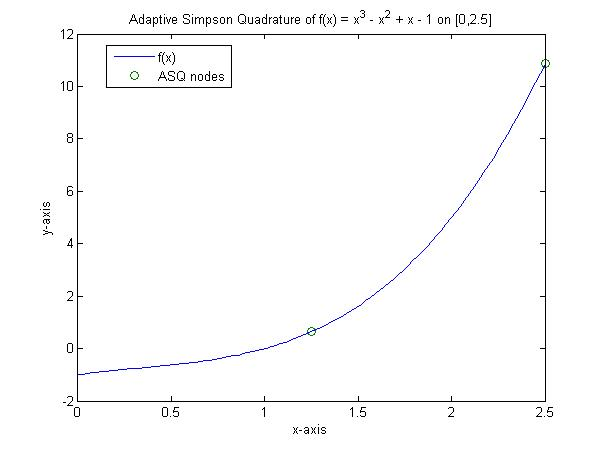
\includegraphics[width=450px]{graphics/cubic_integral_adaptive_simps.jpg}
  \caption[ASQ applied to a cubic function]{ASQ applied to a cubic function. Simpson's rule obtains an exact value for this integral, so the adaptive rule does not 
  have to subdivide the interval at all.}
\end{figure}

\begin{figure}[H]
  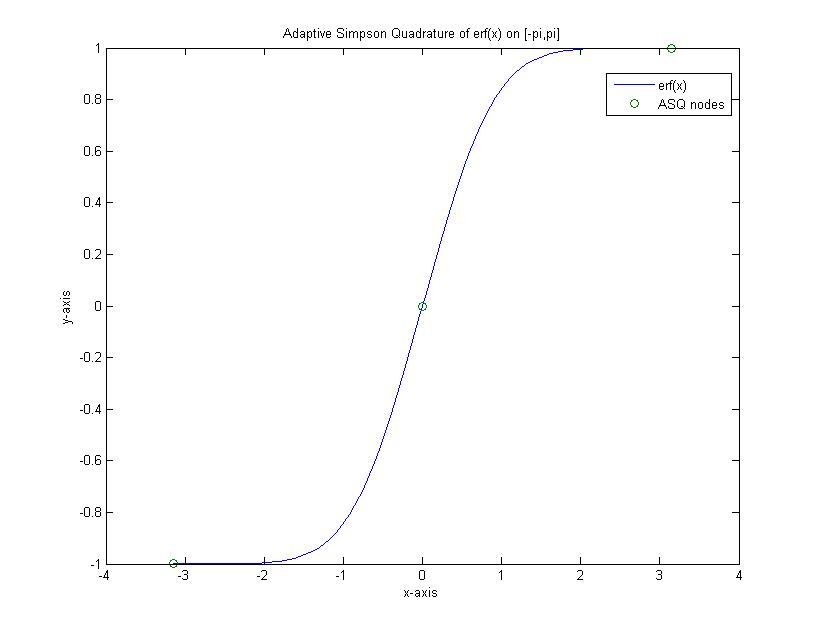
\includegraphics[width=550px]{graphics/erf_adaptive_simps1.jpg}
  \caption[ASQ applied to the error function on a symmetric interval]{ASQ applied to the error function on a symmetric interval. As a consequence of the symmetry of this function about zero,
  the adaptive scheme finds the value of the integral--zero--without subdivision.}
\end{figure}

\begin{figure}[H]
\centering
  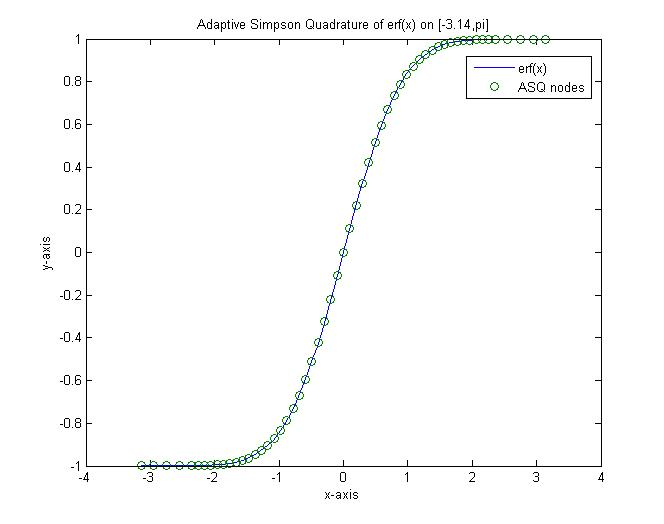
\includegraphics[width=550px]{graphics/erf_adaptive_simps2.jpg}
  \caption[ASQ applied to the error function on an asymmetric interval]{ASQ applied to the error function on an asymmetric interval. By shifting the values of the endpoints slightly we break the symmetry, and now ASQ needs many subdivisions to find a satisfactory approximation. Perhaps surprisingly, slightly more intervals are needed where the values of the function change the least. See the next section for the results of CSQ on this function.}
\end{figure}

\begin{figure}[H]
\centering
  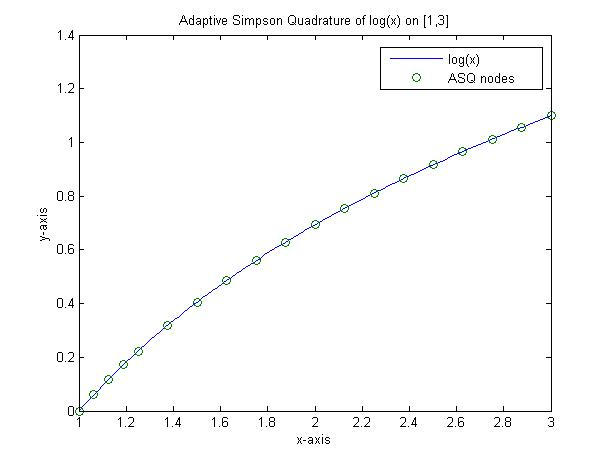
\includegraphics[width=450px]{graphics/log_adaptive_simps.jpg}
  \caption[ASQ applied to the natural logarithm]{ASQ applied to the natural logarithm. For particularly well-behaved integrals, the intervals found by ASQ end up being evenly-spaced or close to it.}
\end{figure}

\begin{figure}[H]
  \centering
  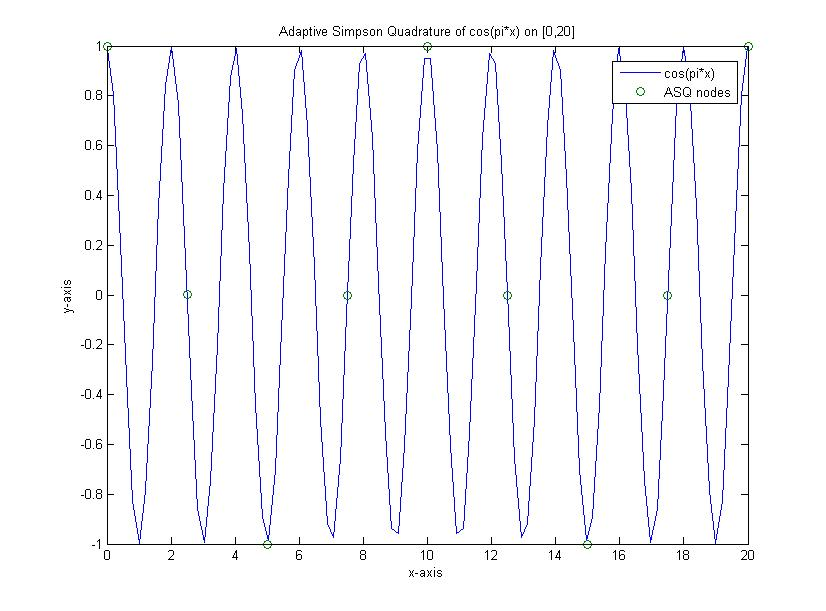
\includegraphics[width=500px]{graphics/cospix_adaptive_simps.jpg}
  \caption[ASQ applied to $\cos(\pi x)$]{ASQ applied to $\cos(\pi x)$. Ultimately, ASQ finds evenly-spaced intervals. However, one easily sees why evenly-spaced intervals chosen \textit{a priori} could become a problem when numerically integrating a periodic function. Compare this figure to the next.}
\end{figure}

\begin{figure}[H]
  \centering
  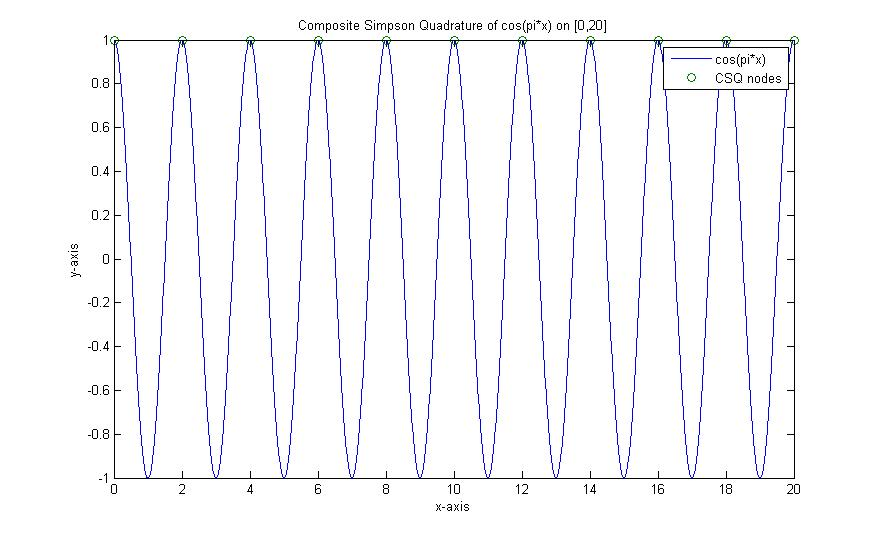
\includegraphics[width=500px]{graphics/cospix_composite_simps.jpg}
  \caption[CSQ applied to $\cos(\pi x)$]{CSQ applied to $\cos(\pi x)$. By carelessly selecting evenly-spaced intervals for composite Simpson quadrature, we accidentally chose the crest of every wave as the sampling point! Refer to Tables 1 and 2 for numerical data on this integral.}
\end{figure}
\end{center}